% Options for packages loaded elsewhere
\PassOptionsToPackage{unicode}{hyperref}
\PassOptionsToPackage{hyphens}{url}
%
\documentclass[
  11pt,
  ignorenonframetext,
]{beamer}
\usepackage{pgfpages}
\setbeamertemplate{caption}[numbered]
\setbeamertemplate{caption label separator}{: }
\setbeamercolor{caption name}{fg=normal text.fg}
\beamertemplatenavigationsymbolsempty
% Prevent slide breaks in the middle of a paragraph
\widowpenalties 1 10000
\raggedbottom
\setbeamertemplate{part page}{
  \centering
  \begin{beamercolorbox}[sep=16pt,center]{part title}
    \usebeamerfont{part title}\insertpart\par
  \end{beamercolorbox}
}
\setbeamertemplate{section page}{
  \centering
  \begin{beamercolorbox}[sep=12pt,center]{part title}
    \usebeamerfont{section title}\insertsection\par
  \end{beamercolorbox}
}
\setbeamertemplate{subsection page}{
  \centering
  \begin{beamercolorbox}[sep=8pt,center]{part title}
    \usebeamerfont{subsection title}\insertsubsection\par
  \end{beamercolorbox}
}
\AtBeginPart{
  \frame{\partpage}
}
\AtBeginSection{
  \ifbibliography
  \else
    \frame{\sectionpage}
  \fi
}
\AtBeginSubsection{
  \frame{\subsectionpage}
}

\usepackage{amsmath,amssymb}
\usepackage{iftex}
\ifPDFTeX
  \usepackage[T1]{fontenc}
  \usepackage[utf8]{inputenc}
  \usepackage{textcomp} % provide euro and other symbols
\else % if luatex or xetex
  \usepackage{unicode-math}
  \defaultfontfeatures{Scale=MatchLowercase}
  \defaultfontfeatures[\rmfamily]{Ligatures=TeX,Scale=1}
\fi
\usepackage{lmodern}
\usetheme[]{AnnArbor}
\usecolortheme{seahorse}
\ifPDFTeX\else  
    % xetex/luatex font selection
\fi
% Use upquote if available, for straight quotes in verbatim environments
\IfFileExists{upquote.sty}{\usepackage{upquote}}{}
\IfFileExists{microtype.sty}{% use microtype if available
  \usepackage[]{microtype}
  \UseMicrotypeSet[protrusion]{basicmath} % disable protrusion for tt fonts
}{}
\makeatletter
\@ifundefined{KOMAClassName}{% if non-KOMA class
  \IfFileExists{parskip.sty}{%
    \usepackage{parskip}
  }{% else
    \setlength{\parindent}{0pt}
    \setlength{\parskip}{6pt plus 2pt minus 1pt}}
}{% if KOMA class
  \KOMAoptions{parskip=half}}
\makeatother
\usepackage{xcolor}
\newif\ifbibliography
\setlength{\emergencystretch}{3em} % prevent overfull lines
\setcounter{secnumdepth}{5}

\usepackage{color}
\usepackage{fancyvrb}
\newcommand{\VerbBar}{|}
\newcommand{\VERB}{\Verb[commandchars=\\\{\}]}
\DefineVerbatimEnvironment{Highlighting}{Verbatim}{commandchars=\\\{\}}
% Add ',fontsize=\small' for more characters per line
\usepackage{framed}
\definecolor{shadecolor}{RGB}{241,243,245}
\newenvironment{Shaded}{\begin{snugshade}}{\end{snugshade}}
\newcommand{\AlertTok}[1]{\textcolor[rgb]{0.68,0.00,0.00}{#1}}
\newcommand{\AnnotationTok}[1]{\textcolor[rgb]{0.37,0.37,0.37}{#1}}
\newcommand{\AttributeTok}[1]{\textcolor[rgb]{0.40,0.45,0.13}{#1}}
\newcommand{\BaseNTok}[1]{\textcolor[rgb]{0.68,0.00,0.00}{#1}}
\newcommand{\BuiltInTok}[1]{\textcolor[rgb]{0.00,0.23,0.31}{#1}}
\newcommand{\CharTok}[1]{\textcolor[rgb]{0.13,0.47,0.30}{#1}}
\newcommand{\CommentTok}[1]{\textcolor[rgb]{0.37,0.37,0.37}{#1}}
\newcommand{\CommentVarTok}[1]{\textcolor[rgb]{0.37,0.37,0.37}{\textit{#1}}}
\newcommand{\ConstantTok}[1]{\textcolor[rgb]{0.56,0.35,0.01}{#1}}
\newcommand{\ControlFlowTok}[1]{\textcolor[rgb]{0.00,0.23,0.31}{#1}}
\newcommand{\DataTypeTok}[1]{\textcolor[rgb]{0.68,0.00,0.00}{#1}}
\newcommand{\DecValTok}[1]{\textcolor[rgb]{0.68,0.00,0.00}{#1}}
\newcommand{\DocumentationTok}[1]{\textcolor[rgb]{0.37,0.37,0.37}{\textit{#1}}}
\newcommand{\ErrorTok}[1]{\textcolor[rgb]{0.68,0.00,0.00}{#1}}
\newcommand{\ExtensionTok}[1]{\textcolor[rgb]{0.00,0.23,0.31}{#1}}
\newcommand{\FloatTok}[1]{\textcolor[rgb]{0.68,0.00,0.00}{#1}}
\newcommand{\FunctionTok}[1]{\textcolor[rgb]{0.28,0.35,0.67}{#1}}
\newcommand{\ImportTok}[1]{\textcolor[rgb]{0.00,0.46,0.62}{#1}}
\newcommand{\InformationTok}[1]{\textcolor[rgb]{0.37,0.37,0.37}{#1}}
\newcommand{\KeywordTok}[1]{\textcolor[rgb]{0.00,0.23,0.31}{#1}}
\newcommand{\NormalTok}[1]{\textcolor[rgb]{0.00,0.23,0.31}{#1}}
\newcommand{\OperatorTok}[1]{\textcolor[rgb]{0.37,0.37,0.37}{#1}}
\newcommand{\OtherTok}[1]{\textcolor[rgb]{0.00,0.23,0.31}{#1}}
\newcommand{\PreprocessorTok}[1]{\textcolor[rgb]{0.68,0.00,0.00}{#1}}
\newcommand{\RegionMarkerTok}[1]{\textcolor[rgb]{0.00,0.23,0.31}{#1}}
\newcommand{\SpecialCharTok}[1]{\textcolor[rgb]{0.37,0.37,0.37}{#1}}
\newcommand{\SpecialStringTok}[1]{\textcolor[rgb]{0.13,0.47,0.30}{#1}}
\newcommand{\StringTok}[1]{\textcolor[rgb]{0.13,0.47,0.30}{#1}}
\newcommand{\VariableTok}[1]{\textcolor[rgb]{0.07,0.07,0.07}{#1}}
\newcommand{\VerbatimStringTok}[1]{\textcolor[rgb]{0.13,0.47,0.30}{#1}}
\newcommand{\WarningTok}[1]{\textcolor[rgb]{0.37,0.37,0.37}{\textit{#1}}}

\providecommand{\tightlist}{%
  \setlength{\itemsep}{0pt}\setlength{\parskip}{0pt}}\usepackage{longtable,booktabs,array}
\usepackage{calc} % for calculating minipage widths
\usepackage{caption}
% Make caption package work with longtable
\makeatletter
\def\fnum@table{\tablename~\thetable}
\makeatother
\usepackage{graphicx}
\makeatletter
\def\maxwidth{\ifdim\Gin@nat@width>\linewidth\linewidth\else\Gin@nat@width\fi}
\def\maxheight{\ifdim\Gin@nat@height>\textheight\textheight\else\Gin@nat@height\fi}
\makeatother
% Scale images if necessary, so that they will not overflow the page
% margins by default, and it is still possible to overwrite the defaults
% using explicit options in \includegraphics[width, height, ...]{}
\setkeys{Gin}{width=\maxwidth,height=\maxheight,keepaspectratio}
% Set default figure placement to htbp
\makeatletter
\def\fps@figure{htbp}
\makeatother

\usepackage{booktabs}
\usepackage{longtable}
\usepackage{array}
\usepackage{multirow}
\usepackage{wrapfig}
\usepackage{float}
\usepackage{colortbl}
\usepackage{pdflscape}
\usepackage{tabu}
\usepackage{threeparttable}
\usepackage{threeparttablex}
\usepackage[normalem]{ulem}
\usepackage{makecell}
\usepackage{xcolor}
\usepackage{amsmath, amssymb, bbm, amstext, array, listings, mathtools, caption, color, graphics, ulem, caption, changepage, atbegshi, soul}
\newcommand\E{\mathbb{E}}
\newcommand\V{\mathbb{V}}
\hypersetup{colorlinks=true,linkcolor=red}
\usepackage{ulem}
\pdfstringdefDisableCommands{\let\sout\relax}
\makeatletter
\makeatother
\makeatletter
\makeatother
\makeatletter
\@ifpackageloaded{caption}{}{\usepackage{caption}}
\AtBeginDocument{%
\ifdefined\contentsname
  \renewcommand*\contentsname{Table of contents}
\else
  \newcommand\contentsname{Table of contents}
\fi
\ifdefined\listfigurename
  \renewcommand*\listfigurename{List of Figures}
\else
  \newcommand\listfigurename{List of Figures}
\fi
\ifdefined\listtablename
  \renewcommand*\listtablename{List of Tables}
\else
  \newcommand\listtablename{List of Tables}
\fi
\ifdefined\figurename
  \renewcommand*\figurename{Figure}
\else
  \newcommand\figurename{Figure}
\fi
\ifdefined\tablename
  \renewcommand*\tablename{Table}
\else
  \newcommand\tablename{Table}
\fi
}
\@ifpackageloaded{float}{}{\usepackage{float}}
\floatstyle{ruled}
\@ifundefined{c@chapter}{\newfloat{codelisting}{h}{lop}}{\newfloat{codelisting}{h}{lop}[chapter]}
\floatname{codelisting}{Listing}
\newcommand*\listoflistings{\listof{codelisting}{List of Listings}}
\makeatother
\makeatletter
\@ifpackageloaded{caption}{}{\usepackage{caption}}
\@ifpackageloaded{subcaption}{}{\usepackage{subcaption}}
\makeatother
\makeatletter
\@ifpackageloaded{tcolorbox}{}{\usepackage[skins,breakable]{tcolorbox}}
\makeatother
\makeatletter
\@ifundefined{shadecolor}{\definecolor{shadecolor}{rgb}{.97, .97, .97}}
\makeatother
\makeatletter
\makeatother
\makeatletter
\makeatother
\ifLuaTeX
  \usepackage{selnolig}  % disable illegal ligatures
\fi
\IfFileExists{bookmark.sty}{\usepackage{bookmark}}{\usepackage{hyperref}}
\IfFileExists{xurl.sty}{\usepackage{xurl}}{} % add URL line breaks if available
\urlstyle{same} % disable monospaced font for URLs
\hypersetup{
  pdftitle={Lectures on causal inference and experimental methods},
  pdfauthor={Macartan Humphreys},
  hidelinks,
  pdfcreator={LaTeX via pandoc}}

\title{Lectures on causal inference and experimental methods}
\author{Macartan Humphreys}
\date{}

\begin{document}
\frame{\titlepage}
\ifdefined\Shaded\renewenvironment{Shaded}{\begin{tcolorbox}[borderline west={3pt}{0pt}{shadecolor}, frame hidden, interior hidden, boxrule=0pt, sharp corners, enhanced, breakable]}{\end{tcolorbox}}\fi

\hypertarget{frequentist-analysis}{%
\section{\texorpdfstring{Frequentist Analysis
\label{L_inference}}{Frequentist Analysis }}\label{frequentist-analysis}}

\begin{frame}{Frequentist Analysis \label{L_inference}}
\hyperlink{ideas}{\beamergotobutton{Top}}
\end{frame}

\hypertarget{basic-analysis}{%
\subsection{\texorpdfstring{Basic Analysis
\label{nools}}{Basic Analysis }}\label{basic-analysis}}

\begin{frame}{ATE}
\protect\hypertarget{ate}{}
Unbiased estimates of the (sample) average treatment effect can be
estimated (\textbf{whether or not there imbalance on covariates}) using:
\[
\widehat{ATE} = \frac{1}{n_T}\sum_TY_i - \frac{1}{n_C}\sum_CY_i,
\]

Say different strata or blocks \(\mathcal{S}\) had different assignment
probabilities. Then you could estimate:

\begin{equation} \widehat{ATE} = \sum_{S\in \mathcal{S}}\frac{n_{S}}{n} \left(\frac{1}{n_{S1}}\sum_{S\cap T}y_i - \frac{1}{n_{S0}}\sum_{S\cap C}y_i \right) \end{equation}

Which also corresponds to the difference in the weighted average of
treatment outcomes (with weights given by the inverse of the probability
that each unit is assigend to treatment) and control outcomes (with
weights given by the inverse of the probability that each unit is
assigend to control).
\end{frame}

\begin{frame}{ATE with IPW}
\protect\hypertarget{ate-with-ipw}{}
\begin{itemize}
\item
  The average difference in means estiamator is the same as what you
  would get if you weighted inversely by shares of units in different
  conditions inside blocks.
\item
  But \textbf{inverse propensity weighting} is a more general principle,
  which can be used even if you do not have blocks.
\item
  The intuition for it comes stright from \textbf{sampling weights} ---
  you weight up in order to recover an unbiased estiamte of the
  potential outcomes for all units, whether or not they are assigned to
  treatment.
\item
  With sampling weights however you can include units even if their
  weight was 1. \emph{Why can you not include these units when doing
  inverse propensity weighting?}
\end{itemize}
\end{frame}

\begin{frame}{Illustration: Estimating treatment effects with terrible
treatment assignments: Fixer\label{Fixer}}
\protect\hypertarget{illustration-estimating-treatment-effects-with-terrible-treatment-assignments-fixer}{}
\footnotesize

Say you made a mess and used a randomization that was correlated with
some variable, \(X\). For example:

\begin{itemize}
\tightlist
\item
  The randomization is done in a way that introduces a correlation
  between Treatment Assignment and Potential Outcomes
\item
  Then possibly, even though there is no true causal effect, we naively
  estimate a large one --- enormous bias
\item
  However since we know the assignment procedure we can \textbf{fully}
  correct for the bias
\item
  In the next example, we do this using ``\textbf{inverse propensity
  score weighting}.'' This is exactly analogous to standard survey
  weighting --- since we selected different units for treatment with
  different probabilities, we weight them differently to recover the
  average outcome among treated units (same for control).
\end{itemize}
\end{frame}

\begin{frame}[fragile]{Basic randomization: Fixer}
\protect\hypertarget{basic-randomization-fixer}{}
Code to generate bad assignment but proper propensity weights:

\begin{Shaded}
\begin{Highlighting}[]
\CommentTok{\# design \textless{}{-} }
\CommentTok{\#   declare\_model(N = 200,}
\CommentTok{\#                 X = runif(N),}
\CommentTok{\#                 Y0 = X,}
\CommentTok{\#                 Y1 = X,}
\CommentTok{\#                 Y = X)}

\NormalTok{n  }\OtherTok{\textless{}{-}} \DecValTok{200}\NormalTok{; reps }\OtherTok{\textless{}{-}} \DecValTok{500}\NormalTok{; X  }\OtherTok{\textless{}{-}} \FunctionTok{runif}\NormalTok{(n)     }\CommentTok{\# Create a covariate (length n)}
\NormalTok{Y  }\OtherTok{\textless{}{-}}\NormalTok{ Y1 }\OtherTok{\textless{}{-}}\NormalTok{ Y0 }\OtherTok{\textless{}{-}}\NormalTok{ X                        }\CommentTok{\# Say X completely determines Y!}
\NormalTok{Z  }\OtherTok{\textless{}{-}} \ControlFlowTok{function}\NormalTok{(i) }\FunctionTok{rank}\NormalTok{(X}\SpecialCharTok{+}\DecValTok{2}\SpecialCharTok{*}\FunctionTok{runif}\NormalTok{(n))}\SpecialCharTok{\textgreater{}}\NormalTok{(n}\SpecialCharTok{/}\DecValTok{2}\NormalTok{) }\CommentTok{\# Bad randomization! }
\NormalTok{P  }\OtherTok{\textless{}{-}} \FunctionTok{sapply}\NormalTok{(}\DecValTok{1}\SpecialCharTok{:}\NormalTok{reps, Z)                    }\CommentTok{\# Lots of possible draws}
\NormalTok{p  }\OtherTok{\textless{}{-}} \FunctionTok{apply}\NormalTok{(P, }\DecValTok{1}\NormalTok{, mean)                    }\CommentTok{\# Recreate propensities!}
\NormalTok{pw }\OtherTok{\textless{}{-}}\NormalTok{ (}\SpecialCharTok{!}\NormalTok{P)}\SpecialCharTok{*}\NormalTok{(}\DecValTok{1}\SpecialCharTok{/}\NormalTok{(}\DecValTok{1}\SpecialCharTok{{-}}\NormalTok{p)); pw[P]}\OtherTok{=}\NormalTok{(P}\SpecialCharTok{*}\NormalTok{(}\DecValTok{1}\SpecialCharTok{/}\NormalTok{p))[P]   }\CommentTok{\# Create inv prop weights}

\NormalTok{naive   }\OtherTok{\textless{}{-}} \FunctionTok{sapply}\NormalTok{(}\DecValTok{1}\SpecialCharTok{:}\FunctionTok{ncol}\NormalTok{(P),}\ControlFlowTok{function}\NormalTok{(i) \{}
              \FunctionTok{mean}\NormalTok{(Y[P[,i]])}\SpecialCharTok{{-}}\FunctionTok{mean}\NormalTok{(Y[}\SpecialCharTok{!}\NormalTok{P[,i]])\}) }
\NormalTok{weightd }\OtherTok{\textless{}{-}} \FunctionTok{sapply}\NormalTok{(}\DecValTok{1}\SpecialCharTok{:}\FunctionTok{ncol}\NormalTok{(P),}\ControlFlowTok{function}\NormalTok{(i) \{  }\CommentTok{\# IPW estimates}
              \FunctionTok{weighted.mean}\NormalTok{(Y[P[,i]],  pw[,i][P[,i]])}\SpecialCharTok{{-}}
              \FunctionTok{weighted.mean}\NormalTok{(Y[}\SpecialCharTok{!}\NormalTok{P[,i]], pw[,i][}\SpecialCharTok{!}\NormalTok{P[,i]])\}) }
\end{Highlighting}
\end{Shaded}
\end{frame}

\begin{frame}{Basic randomization: Fixer}
\protect\hypertarget{basic-randomization-fixer-1}{}
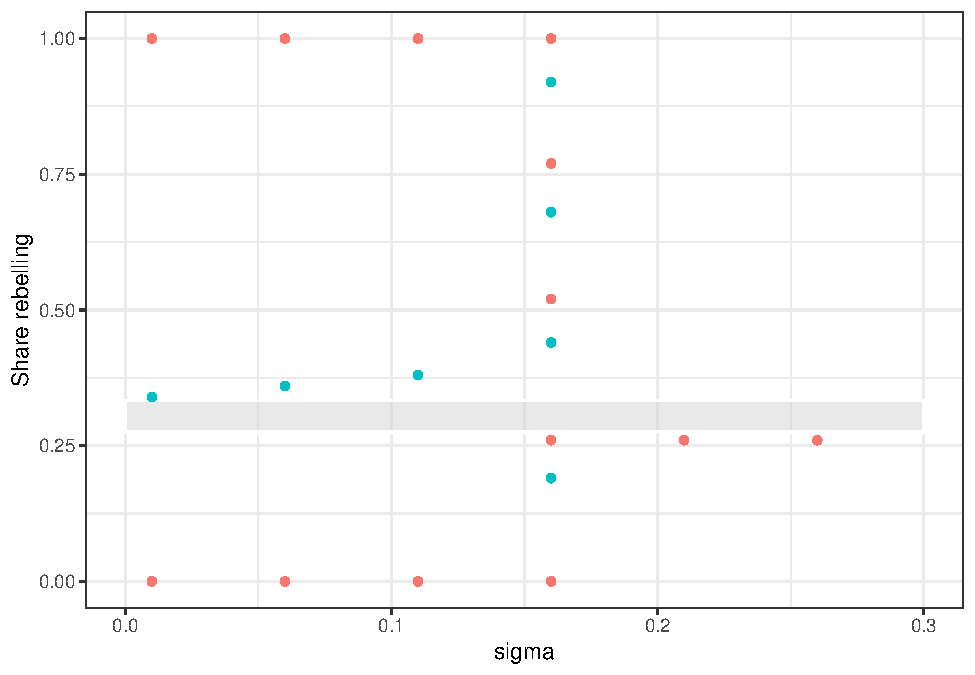
\includegraphics{3.1_fisher_files/figure-beamer/unnamed-chunk-3-1.pdf}
\end{frame}

\begin{frame}{IPW with one unit!}
\protect\hypertarget{ipw-with-one-unit}{}
This example is surprising but it helps you see the logic of why inverse
weighting gets unbiased estimates (and why that might not guarantee a
reasonable answer)

Imagine there is one unit with potential outcomes
\(Y(1) = 2, Y(0) = 1\). So the unit level treatment effect is 1.

You toss a coin.

\begin{itemize}
\tightlist
\item
  If you assign to treatment you estimate:
  \(\hat\tau = \frac{2}{0.5} = 4\)
\item
  If you assign to control you estimate:
  \(\hat\tau = -\frac{1}{0.5} = -2\)
\end{itemize}

SO your expected estimate is: \[0.5 \times 4 - 0.5 \times (-2) = 1\]

Great on average but always lousy
\end{frame}

\hypertarget{design-based-estimation-of-variance}{%
\subsection{Design Based Estimation of
Variance}\label{design-based-estimation-of-variance}}

\begin{frame}{Var(ATE)}
\protect\hypertarget{varate}{}
\begin{itemize}
\tightlist
\item
  Recall that the treatment effect is gotten by taking a sample of
  outcomes under treatment and comparing them to a sample of outcomes
  under control
\item
  Say that there is no ``error''
\item
  Why would this procedure produce uncertainty?
\end{itemize}
\end{frame}

\begin{frame}{Var(ATE)}
\protect\hypertarget{varate-1}{}
\begin{itemize}
\tightlist
\item
  Why would this procedure produce uncertainty?
\item
  The uncertainty comes from being uncertain about the average outcome
  under control from observations of the control units, and from being
  uncertain about the average outcome under treatment from obervation of
  the treated units
\item
  In other words, it comes from the variance in the treatment outcomes
  and variance in the control outcomes (and not, for example, from
  variance in the treatment effect)
\end{itemize}
\end{frame}

\begin{frame}{Var(ATE)}
\protect\hypertarget{varate-2}{}
\scriptsize You can also estimate variance straight from the data. From
\href{http://www.stat.berkeley.edu/~census/neyregcm.pdf}{Freedman Prop 1}
(using combinatorics!) we have:

\begin{eqnarray*} 
V(\widehat{ATE})  &=  &\frac{1}{n-1}\left[\frac{n_C}{n_T}V(Y(1)) +  \frac{n_T}{n_C}V(Y(0))\right] + 2C\left(Y(1),Y(0)\right)  \nonumber \\
\end{eqnarray*} Usefully rewritten as: \begin{eqnarray*} 
V(\widehat{ATE})  &=  &\frac{n}{n-1}\left[\frac{V(Y(1))}{n_T} +  \frac{V(Y(0))}{n_C}\right] - \frac{1}{n-1}\left[V(Y(1)) + V(Y(0)) - 2C\left(Y(1),Y(0)\right)\right]  \nonumber 
\end{eqnarray*}

\dots where \(V\) denotes variance and \(C\) covariance

Note:

\begin{itemize} \scriptsize
\item We can use the sample estimates $s^2(\{Y_i\}_{i \in C})$ and $s^2(\{Y_i\}_{i \in T})$ for the first part.
\item But $C(Y(1),Y(0))$ cannot be estimated from data.
\item The ``\textbf{Neyman}'' estimator ignores the second part (and so is conservative).
\item Tip: for STATA users, use ``, robust'' (see Samii and Aronow: On equivalencies between design-based and regression-based variance estimators for randomized experiments)
\end{itemize}
\end{frame}

\begin{frame}{ATE and Var(ATE)\}}
\protect\hypertarget{ate-and-varate}{}
For the case with blocking, the conservative estimator is:

\begin{equation*} V(\widehat{ATE})   = {\sum_{S\in \mathcal{S}}{\left(\frac{n_{S}}{n}\right)^2} \left({\frac{s^2_{S1}}{n_{S1}}} + {\frac{s^2_{S0}}{n_{S0}}} \right)}  \end{equation*}

Skip to \hyperlink{CA}{\beamergotobutton{Covariate Adjustment}} or
\hyperlink{ideas}{\beamerreturnbutton{Big Ideas}}
\end{frame}

\begin{frame}{Illustration of Neyman Conservative Estimator}
\protect\hypertarget{illustration-of-neyman-conservative-estimator}{}
An illustration of \textit{how} conservative the conservative estimator
of variance really is (numbers in plot are correlations between \(Y(1)\)
and \(Y(0)\).

We confirm that:

\begin{enumerate}
\tightlist
\item
  the estimator is conservative
\item
  the estimator is more conservative for negative correlations between
  \(Y(0)\) and \(Y(1)\) --- eg if those cases that do particularly badly
  in control are the ones that do particularly well in treatment \%, and
\item
  with \(\tau\) and \(V(Y(0))\) fixed. high positive correlations are
  associated with highest variance.
\end{enumerate}
\end{frame}

\begin{frame}{Illustration of Neyman Conservative Estimator}
\protect\hypertarget{illustration-of-neyman-conservative-estimator-1}{}
\includegraphics{3.1_fisher_files/figure-beamer/unnamed-chunk-5-1.pdf}
\end{frame}

\begin{frame}{Illustration of Neyman Conservative Estimator}
\protect\hypertarget{illustration-of-neyman-conservative-estimator-2}{}
\begin{longtable}[]{@{}
  >{\raggedright\arraybackslash}p{(\columnwidth - 12\tabcolsep) * \real{0.0567}}
  >{\raggedright\arraybackslash}p{(\columnwidth - 12\tabcolsep) * \real{0.0567}}
  >{\raggedright\arraybackslash}p{(\columnwidth - 12\tabcolsep) * \real{0.1489}}
  >{\raggedright\arraybackslash}p{(\columnwidth - 12\tabcolsep) * \real{0.0709}}
  >{\raggedright\arraybackslash}p{(\columnwidth - 12\tabcolsep) * \real{0.1348}}
  >{\raggedright\arraybackslash}p{(\columnwidth - 12\tabcolsep) * \real{0.2057}}
  >{\raggedright\arraybackslash}p{(\columnwidth - 12\tabcolsep) * \real{0.3262}}@{}}
\toprule\noalign{}
\begin{minipage}[b]{\linewidth}\raggedright
\(\tau\)
\end{minipage} & \begin{minipage}[b]{\linewidth}\raggedright
\(\rho\)
\end{minipage} & \begin{minipage}[b]{\linewidth}\raggedright
\(\sigma^2_{Y(1)}\)
\end{minipage} & \begin{minipage}[b]{\linewidth}\raggedright
\(\Delta\)
\end{minipage} & \begin{minipage}[b]{\linewidth}\raggedright
\(\sigma^2_{\tau}\)
\end{minipage} & \begin{minipage}[b]{\linewidth}\raggedright
\(\widehat{\sigma}^2_{\tau}\)
\end{minipage} & \begin{minipage}[b]{\linewidth}\raggedright
\(\widehat{\sigma}^2_{\tau(\text{Neyman})}\)
\end{minipage} \\
\midrule\noalign{}
\endhead
1.00 & -1.00 & 1.00 & -0.04 & 0.00 & -0.00 & 0.04 \\
1.00 & -0.67 & 1.00 & -0.03 & 0.01 & 0.01 & 0.04 \\
1.00 & -0.33 & 1.00 & -0.03 & 0.01 & 0.01 & 0.04 \\
1.00 & 0.00 & 1.00 & -0.02 & 0.02 & 0.02 & 0.04 \\
1.00 & 0.33 & 1.00 & -0.01 & 0.03 & 0.03 & 0.04 \\
1.00 & 0.67 & 1.00 & -0.01 & 0.03 & 0.03 & 0.04 \\
1.00 & 1.00 & 1.00 & 0.00 & 0.04 & 0.04 & 0.04 \\
\bottomrule\noalign{}
\end{longtable}

Here \(\rho\) is the unobserved correlation between \(Y(1)\) and
\(Y(0)\); and \(\Delta\) is the final term in the sample variance
equation that we cannot estimate.
\end{frame}

\begin{frame}{Tighter Bounds On Variance Estimate}
\protect\hypertarget{tighter-bounds-on-variance-estimate}{}
The conservative variance comes from the fact that you do not know the
covariance between \(Y(1)\) and \(Y(0)\).

\begin{itemize}
\tightlist
\item
  But as
  \href{http://arxiv.org/pdf/1405.6555.pdf}{Aronow, Green, and Lee (2014)}
  point out, you \textit{do} know something.
\item
  Intuitively, if you know that the variance of \(Y(1)\) is 0, then the
  covariance also has to be zero.
\item
  This basic insight opens a way of calculating bounds on the variance
  of the sample average treatment effect.
\end{itemize}
\end{frame}

\begin{frame}{Tighter Bounds On Variance Estimate}
\protect\hypertarget{tighter-bounds-on-variance-estimate-1}{}
Example:

\begin{itemize}
\tightlist
\item
  Take a million-observation dataset, with treatment randomly assigned
\item
  Assume \(Y(0)=0\) for everyone and \(Y(1)\) distributed normally with
  mean 0 and standard deviation of 1000.
\item
  Note here the covariance of \(Y(1)\) and \(Y(0)\) is 0.
\item
  Note the true variance of the estimated sample average treatment
  effect should be (approx)
  \(\frac{Var(Y(1))}{\sqrt{1000000}} + \frac{Var(Y(0))}{\sqrt{1000000}} = 1\).
\item
  But using the Neyman estimator (or OLS!) we estimate (approx)
  \(\frac{Var(Y(1))}{\sqrt{1000000/2}} + \frac{Var(Y(0))}{\sqrt{1000000/2}} = \sqrt{2}\).
\item
  But we can recover the truth knowing the covariance between \(Y(1)\)
  and \(Y(0)\) is 0.
\end{itemize}
\end{frame}

\begin{frame}[fragile]{Tighter Bounds On Variance Estimate: Code}
\protect\hypertarget{tighter-bounds-on-variance-estimate-code}{}
\begin{Shaded}
\begin{Highlighting}[]
\NormalTok{sharp\_var }\OtherTok{\textless{}{-}} \ControlFlowTok{function}\NormalTok{(yt,yc,}\AttributeTok{N=}\FunctionTok{length}\NormalTok{(}\FunctionTok{c}\NormalTok{(yt,yc)),}\AttributeTok{upper=}\ConstantTok{TRUE}\NormalTok{)\{}
\NormalTok{ m }\OtherTok{\textless{}{-}} \FunctionTok{length}\NormalTok{(yt);  n }\OtherTok{\textless{}{-}}\NormalTok{ m }\SpecialCharTok{+} \FunctionTok{length}\NormalTok{(yc)}
\NormalTok{ V }\OtherTok{\textless{}{-}} \ControlFlowTok{function}\NormalTok{(x,N) \{}
\NormalTok{       (N}\DecValTok{{-}1}\NormalTok{)}\SpecialCharTok{/}\NormalTok{(N}\SpecialCharTok{*}\NormalTok{(}\FunctionTok{length}\NormalTok{(x)}\SpecialCharTok{{-}}\DecValTok{1}\NormalTok{)) }\SpecialCharTok{*} \FunctionTok{sum}\NormalTok{((x }\SpecialCharTok{{-}} \FunctionTok{mean}\NormalTok{(x))}\SpecialCharTok{\^{}}\DecValTok{2}\NormalTok{)\}}
\NormalTok{ yt }\OtherTok{\textless{}{-}} \FunctionTok{sort}\NormalTok{(yt)}
 \ControlFlowTok{if}\NormalTok{(upper) \{yc }\OtherTok{\textless{}{-}} \FunctionTok{sort}\NormalTok{(yc)}
\NormalTok{       \} }\ControlFlowTok{else}\NormalTok{ \{yc }\OtherTok{\textless{}{-}} \FunctionTok{sort}\NormalTok{(yc,}\AttributeTok{decreasing=}\ConstantTok{TRUE}\NormalTok{)\}}
\NormalTok{ p\_i }\OtherTok{\textless{}{-}} \FunctionTok{unique}\NormalTok{(}\FunctionTok{sort}\NormalTok{(}\FunctionTok{c}\NormalTok{(}\FunctionTok{seq}\NormalTok{(}\DecValTok{0}\NormalTok{,n}\SpecialCharTok{{-}}\NormalTok{m,}\DecValTok{1}\NormalTok{)}\SpecialCharTok{/}\NormalTok{(n}\SpecialCharTok{{-}}\NormalTok{m),}\FunctionTok{seq}\NormalTok{(}\DecValTok{0}\NormalTok{,m,}\DecValTok{1}\NormalTok{)}\SpecialCharTok{/}\NormalTok{m)))}\SpecialCharTok{{-}} 
\NormalTok{        .Machine}\SpecialCharTok{$}\NormalTok{double.eps}\SpecialCharTok{\^{}}\NormalTok{.}\DecValTok{5}
\NormalTok{ p\_i[}\DecValTok{1}\NormalTok{] }\OtherTok{\textless{}{-}}\NormalTok{ .Machine}\SpecialCharTok{$}\NormalTok{double.eps}\SpecialCharTok{\^{}}\NormalTok{.}\DecValTok{5}
\NormalTok{ yti }\OtherTok{\textless{}{-}}\NormalTok{ yt[}\FunctionTok{ceiling}\NormalTok{(p\_i}\SpecialCharTok{*}\NormalTok{m)]; yci }\OtherTok{\textless{}{-}}\NormalTok{ yc[}\FunctionTok{ceiling}\NormalTok{(p\_i}\SpecialCharTok{*}\NormalTok{(n}\SpecialCharTok{{-}}\NormalTok{m))]}
\NormalTok{ p\_i\_minus }\OtherTok{\textless{}{-}} \FunctionTok{c}\NormalTok{(}\ConstantTok{NA}\NormalTok{,p\_i[}\DecValTok{1}\SpecialCharTok{:}\NormalTok{ (}\FunctionTok{length}\NormalTok{(p\_i)}\SpecialCharTok{{-}}\DecValTok{1}\NormalTok{)])}
 \FunctionTok{return}\NormalTok{(((N}\SpecialCharTok{{-}}\NormalTok{m)}\SpecialCharTok{/}\NormalTok{m }\SpecialCharTok{*} \FunctionTok{V}\NormalTok{(yt,N) }\SpecialCharTok{+}\NormalTok{ (N}\SpecialCharTok{{-}}\NormalTok{(n}\SpecialCharTok{{-}}\NormalTok{m))}\SpecialCharTok{/}\NormalTok{(n}\SpecialCharTok{{-}}\NormalTok{m)}\SpecialCharTok{*}\FunctionTok{V}\NormalTok{(yc,N) }\SpecialCharTok{+}
       \DecValTok{2}\SpecialCharTok{*}\FunctionTok{sum}\NormalTok{(((p\_i}\SpecialCharTok{{-}}\NormalTok{p\_i\_minus)}\SpecialCharTok{*}\NormalTok{yti}\SpecialCharTok{*}\NormalTok{yci)[}\DecValTok{2}\SpecialCharTok{:}\FunctionTok{length}\NormalTok{(p\_i)]) }\SpecialCharTok{{-}}
       \DecValTok{2}\SpecialCharTok{*}\FunctionTok{mean}\NormalTok{(yt)}\SpecialCharTok{*}\FunctionTok{mean}\NormalTok{(yc))}\SpecialCharTok{/}\NormalTok{(N}\DecValTok{{-}1}\NormalTok{))\}}
\end{Highlighting}
\end{Shaded}
\end{frame}

\begin{frame}[fragile]{Illustration}
\protect\hypertarget{illustration}{}
\begin{Shaded}
\begin{Highlighting}[]
\NormalTok{n   }\OtherTok{\textless{}{-}} \DecValTok{1000000}
\NormalTok{Y   }\OtherTok{\textless{}{-}} \FunctionTok{c}\NormalTok{(}\FunctionTok{rep}\NormalTok{(}\DecValTok{0}\NormalTok{,n}\SpecialCharTok{/}\DecValTok{2}\NormalTok{), }\DecValTok{1000}\SpecialCharTok{*}\FunctionTok{rnorm}\NormalTok{(n}\SpecialCharTok{/}\DecValTok{2}\NormalTok{))}
\NormalTok{X   }\OtherTok{\textless{}{-}} \FunctionTok{c}\NormalTok{(}\FunctionTok{rep}\NormalTok{(}\DecValTok{0}\NormalTok{,n}\SpecialCharTok{/}\DecValTok{2}\NormalTok{), }\FunctionTok{rep}\NormalTok{(}\DecValTok{1}\NormalTok{, n}\SpecialCharTok{/}\DecValTok{2}\NormalTok{))}
\NormalTok{ols }\OtherTok{\textless{}{-}} \FunctionTok{round}\NormalTok{(}\FunctionTok{coef}\NormalTok{(}\FunctionTok{summary}\NormalTok{(}\FunctionTok{lm}\NormalTok{(Y}\SpecialCharTok{\textasciitilde{}}\NormalTok{X)))[}\DecValTok{2}\NormalTok{,],}\DecValTok{3}\NormalTok{)}
\FunctionTok{kable}\NormalTok{(}\FunctionTok{t}\NormalTok{(}\FunctionTok{as.matrix}\NormalTok{(ols)))}
\end{Highlighting}
\end{Shaded}

\begin{tabular}{r|r|r|r}
\hline
Estimate & Std. Error & t value & Pr(>|t|)\\
\hline
-0.524 & 1.415 & -0.37 & 0.711\\
\hline
\end{tabular}

\begin{Shaded}
\begin{Highlighting}[]
\NormalTok{sharp }\OtherTok{\textless{}{-}} \FunctionTok{round}\NormalTok{(}\FunctionTok{c}\NormalTok{(}\FunctionTok{sharp\_var}\NormalTok{(Y[X}\SpecialCharTok{==}\DecValTok{1}\NormalTok{], Y[X}\SpecialCharTok{==}\DecValTok{0}\NormalTok{], }\AttributeTok{upper =} \ConstantTok{FALSE}\NormalTok{), }
                 \FunctionTok{sharp\_var}\NormalTok{(Y[X}\SpecialCharTok{==}\DecValTok{1}\NormalTok{], Y[X}\SpecialCharTok{==}\DecValTok{0}\NormalTok{], }\AttributeTok{upper =} \ConstantTok{TRUE}\NormalTok{)),}\DecValTok{3}\NormalTok{)}
\NormalTok{sharp}
\end{Highlighting}
\end{Shaded}

{[}1{]} 1.001 1.001
\end{frame}

\hypertarget{principle-keep-the-reporting-close-to-the-design}{%
\subsection{Principle: Keep the reporting close to the
design}\label{principle-keep-the-reporting-close-to-the-design}}

\begin{frame}{Design based analysis}
\protect\hypertarget{design-based-analysis}{}
\begin{itemize}
    \item  Report the analysis that is implied by the design. 
\bigskip

\begin{table}
\small \centering
\begin{tabular}{cc|ccc|c}\small

           &            &         T2 &            &            &            \\

           &            &          N &          Y &        All &       Diff \\ \hline

        T1 &          N &     \color{blue}$\overline{y}_{00}$ &     \color{blue}$\overline{y}_{01}$ &     $\overline{y}_{0x}$ &    $d_2|T1=0$ \\

           &            &       (sd) &       (sd) &       (sd) &       (sd) \\

           &          Y &     \color{blue}$\overline{y}_{10}$ &     \color{blue}$\overline{y}_{10}$ &         $\overline{y}_{1x}$ &    $d_2|T1=1$ \\

           &            &       (sd) &       (sd) &       (sd) &       (sd) \\

           &        All &     $\overline{y}_{x0}$ &     $\overline{y}_{x1}$ &          $y$ &    \color{red}$d_2$ \\

           &            &       (sd) &       (sd) &       (sd) &       (sd) \\ \hline

           &       Diff &    $d_1|T2=0$ &    $d_1|T2=1$ &    \color{red}$d_1$ &    \color{green} $d_1d_2$ \\

           &            &       (sd) &       (sd) &       (sd) &       (sd) \\

\end{tabular}  
\end{table}
\end{itemize}

\small This is instantly recognizable from the design and returns all
the benefits of the factorial design including all main effects,
conditional causal effects, interactions and summary outcomes. It is
much clearer and more informative than a regression table.
\end{frame}

\hypertarget{covariate-and-regression-adjustment}{%
\subsection{Covariate and Regression
Adjustment}\label{covariate-and-regression-adjustment}}

\begin{frame}{Covariate Adjustment\label{CA}}
\protect\hypertarget{covariate-adjustment}{}
\begin{itemize}
\tightlist
\item
  Even though randomization ensures no bias, you may sometimes
  \textbf{want} to ``\textbf{control}'' for covariates in order to
  improve efficiency (see the discussion of blocking above).
\item
  Or you may \textbf{have} to take account of the fact that the
  assignment to treatment is correlated with a covariate.
\end{itemize}
\end{frame}

\begin{frame}{Covariate Adjustment\label{CA}}
\protect\hypertarget{covariate-adjustment-1}{}
Consider for example this data. \bigskip

\begin{itemize}
\tightlist
\item
  You randomly pair offerers and receivers in a dictator game (in which
  offerers decide how much of \$1 to give to receivers).
\item
  Your population comes from two groups (80\% Baganda and 20\%
  Banyankole) \emph{so in randomly assigning partners you are randomly
  determining whether a partner is a coethnic or not}.
\item
  \textbf{You find that in non-coethnic pairings 35\% is offered, in
  coethnic pairings 48\% is offered.}
\end{itemize}

Should you believe it?
\end{frame}

\begin{frame}{Covariate Adjustment}
\protect\hypertarget{covariate-adjustment-2}{}
\begin{itemize}
\tightlist
\item
  Population: randomly matched Baganda (80\% of pop) and Banyankole
  (20\% of pop)
\item
  You find: in non-coethnic pairings 35\% is offered, in coethnic
  pairings 48\% is offered.
\item
  But a closer look at the data reveals \dots
\end{itemize}

\begin{table}[h!]    \footnotesize
    \begin{tabular}{cc|cc}  \footnotesize
&   &       To: Baganda &To: Banyankole \\ \hline
Offers by   &Baganda    &64\%   & 16\% \\
    &Banyankole &16\%   &4\% \\
    \end{tabular}
    \caption{\small Number of Games}
\end{table}

\begin{table}[h!]    \footnotesize
    \begin{tabular}{cc|cc} \footnotesize
&   &       To: Baganda &To: Banyankole \\ \hline
Offers by   &Baganda    &50 & 50 \\
    &Banyankole &20 &20 \\
    \end{tabular}
    \caption{\small  Average Offers}
\end{table}

\footnotesize So that's a problem
\end{frame}

\begin{frame}{Covariate Adjustment}
\protect\hypertarget{covariate-adjustment-3}{}
Control?

\begin{itemize}
\tightlist
\item
  With such data you might be tempted to `control' for the covariate
  (here: ethnic group), using regression.
\item
  But, perhaps surprisingly, it turns out that regression with
  covariates does not estimate average treatment effects.
\item
  It does estimate an average of treatment effects, but specifically a
  minimum variance estimator, not necessarily an estimator of your
  estimand.
\end{itemize}

Compare:

\begin{itemize}
\tightlist
\item
  \(\hat{\tau}_{ATE} =\sum_{x} \frac{w_x}{\sum_{j}w_{j}}\hat{\tau}_x\)
\item
  \(\hat{\tau}_{OLS} =\sum_{x} \frac{w_xp_x(1-p_x)}{\sum_{j}w_j{p_j(1-p_j)}}\hat{\tau}_x\)
\end{itemize}

Instead the formula above for \(\hat{\tau}_{ATE}\) is all you need to
estimate ATE --- at least for discrete covariates.
\end{frame}

\begin{frame}[fragile]{OLS and its discontents: Illustration}
\protect\hypertarget{ols-and-its-discontents-illustration}{}
Two strata with different potential outcomes and assignment
probabilities.

\begin{itemize}
\tightlist
\item
  Stratum 1 has \(Y(0)=Y(1)=0\) and 1 in 4 are treated
\item
  Stratum 2 has \(Y(1)=14, Y(0)=0\) and 2 in 4 assigned to treatment
\end{itemize}

\begin{Shaded}
\begin{Highlighting}[]
\NormalTok{X   }\OtherTok{\textless{}{-}} \DecValTok{1}\SpecialCharTok{*}\NormalTok{((}\DecValTok{1}\SpecialCharTok{:}\DecValTok{8}\NormalTok{)}\SpecialCharTok{\textgreater{}}\DecValTok{4}\NormalTok{) }\SpecialCharTok{{-}}\NormalTok{ .}\DecValTok{5}
\NormalTok{Z   }\OtherTok{\textless{}{-}} \DecValTok{1}\SpecialCharTok{:}\DecValTok{8}\SpecialCharTok{\%in\%}\FunctionTok{c}\NormalTok{(}\DecValTok{1}\NormalTok{,}\DecValTok{7}\NormalTok{,}\DecValTok{8}\NormalTok{)}
\NormalTok{Y0  }\OtherTok{\textless{}{-}} \FunctionTok{rnorm}\NormalTok{(}\DecValTok{8}\NormalTok{, }\AttributeTok{sd =}\NormalTok{ .}\DecValTok{01}\NormalTok{)}
\NormalTok{Y1  }\OtherTok{\textless{}{-}} \DecValTok{14}\SpecialCharTok{*}\NormalTok{(X}\SpecialCharTok{==}\NormalTok{.}\DecValTok{5}\NormalTok{)}
\NormalTok{Y   }\OtherTok{\textless{}{-}}\NormalTok{ Z}\SpecialCharTok{*}\NormalTok{Y1 }\SpecialCharTok{+}\NormalTok{ (}\DecValTok{1}\SpecialCharTok{{-}}\NormalTok{Z)}\SpecialCharTok{*}\NormalTok{Y0}
\NormalTok{tau }\OtherTok{\textless{}{-}}\NormalTok{ Y1}\SpecialCharTok{{-}}\NormalTok{Y0}
\NormalTok{p   }\OtherTok{\textless{}{-}} \FunctionTok{ave}\NormalTok{(Z, }\AttributeTok{group\_by =}\NormalTok{ X)}
\NormalTok{ipw }\OtherTok{\textless{}{-}} \DecValTok{1}\SpecialCharTok{/}\NormalTok{(p}\SpecialCharTok{*}\NormalTok{Z }\SpecialCharTok{+}\NormalTok{ (}\DecValTok{1}\SpecialCharTok{{-}}\NormalTok{p)}\SpecialCharTok{*}\NormalTok{(}\DecValTok{1}\SpecialCharTok{{-}}\NormalTok{Z))}
\NormalTok{D   }\OtherTok{\textless{}{-}} \FunctionTok{data.frame}\NormalTok{(X, Y0, Y1, Y, tau, p, ipw)}
\end{Highlighting}
\end{Shaded}
\end{frame}

\begin{frame}[fragile]{OLS and its discontents: Illustration}
\protect\hypertarget{ols-and-its-discontents-illustration-1}{}
Two strata with different potential outcomes and assignment
probabilities.

\begin{itemize}
\tightlist
\item
  Stratum 1 has \(Y(0)=Y(1)=0\) and 1 in 4 are treated
\item
  Stratum 2 has \(Y(1)=14, Y(0)=0\) and 2 in 4 assigned to treatment
\end{itemize}

\begin{Shaded}
\begin{Highlighting}[]
\FunctionTok{kable}\NormalTok{(}\FunctionTok{round}\NormalTok{(D,}\DecValTok{3}\NormalTok{))}
\end{Highlighting}
\end{Shaded}

\begin{tabular}{r|r|r|r|r|r|r}
\hline
X & Y0 & Y1 & Y & tau & p & ipw\\
\hline
-0.5 & 0.006 & 0 & 0.000 & -0.006 & 0.25 & 4.000\\
\hline
-0.5 & 0.016 & 0 & 0.016 & -0.016 & 0.25 & 1.333\\
\hline
-0.5 & 0.007 & 0 & 0.007 & -0.007 & 0.25 & 1.333\\
\hline
-0.5 & -0.006 & 0 & -0.006 & 0.006 & 0.25 & 1.333\\
\hline
0.5 & -0.007 & 14 & -0.007 & 14.007 & 0.50 & 2.000\\
\hline
0.5 & -0.004 & 14 & -0.004 & 14.004 & 0.50 & 2.000\\
\hline
0.5 & 0.008 & 14 & 14.000 & 13.992 & 0.50 & 2.000\\
\hline
0.5 & 0.002 & 14 & 14.000 & 13.998 & 0.50 & 2.000\\
\hline
\end{tabular}
\end{frame}

\begin{frame}{OLS and its discontents}
\protect\hypertarget{ols-and-its-discontents}{}
Two strata with different potential outcomes and assignment
probabilities.

\begin{itemize}
\tightlist
\item
  Stratum 1 has \(Y(0)=Y(1)=0\) and 1 in 4 are treated
\item
  Stratum 2 has \(Y(1)=14, Y(0)=0\) and 2 in 4 assigned to treatment.
\end{itemize}

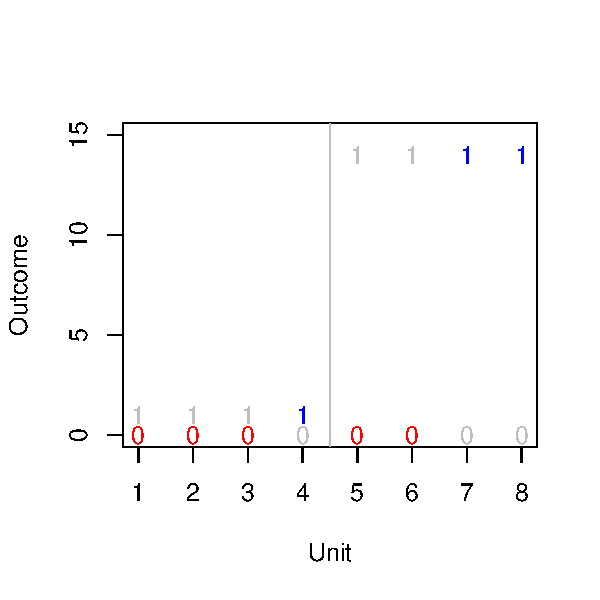
\includegraphics{figs/nools.pdf}
\end{frame}

\begin{frame}[fragile]{OLS and its discontents: Illustration}
\protect\hypertarget{ols-and-its-discontents-illustration-2}{}
Two strata with different potential outcomes and assignment
probabilities.

\begin{Shaded}
\begin{Highlighting}[]
\NormalTok{ols1 }\OtherTok{\textless{}{-}} \FunctionTok{coef}\NormalTok{(}\FunctionTok{summary}\NormalTok{(}\FunctionTok{lm}\NormalTok{(Y}\SpecialCharTok{\textasciitilde{}}\NormalTok{Z, }\AttributeTok{data =}\NormalTok{ D)))[}\DecValTok{2}\NormalTok{,]}
\NormalTok{ols2 }\OtherTok{\textless{}{-}} \FunctionTok{coef}\NormalTok{(}\FunctionTok{summary}\NormalTok{(}\FunctionTok{lm}\NormalTok{(Y}\SpecialCharTok{\textasciitilde{}}\NormalTok{Z}\SpecialCharTok{+}\NormalTok{X, }\AttributeTok{data =}\NormalTok{ D)))[}\DecValTok{2}\NormalTok{,]}
\NormalTok{ipw1 }\OtherTok{\textless{}{-}} \FunctionTok{coef}\NormalTok{(}\FunctionTok{summary}\NormalTok{(}\FunctionTok{lm}\NormalTok{(Y}\SpecialCharTok{\textasciitilde{}}\NormalTok{Z, }\AttributeTok{weight =}\NormalTok{ ipw, }\AttributeTok{data =}\NormalTok{ D)))[}\DecValTok{2}\NormalTok{,]}
\NormalTok{ipw2 }\OtherTok{\textless{}{-}} \FunctionTok{coef}\NormalTok{(}\FunctionTok{summary}\NormalTok{(}\FunctionTok{lm}\NormalTok{(Y}\SpecialCharTok{\textasciitilde{}}\NormalTok{Z}\SpecialCharTok{+}\NormalTok{X, }\AttributeTok{weight =}\NormalTok{ ipw, }\AttributeTok{data =}\NormalTok{ D)))[}\DecValTok{2}\NormalTok{,]}
\NormalTok{sat  }\OtherTok{\textless{}{-}} \FunctionTok{coef}\NormalTok{(}\FunctionTok{summary}\NormalTok{(}\FunctionTok{lm}\NormalTok{(Y}\SpecialCharTok{\textasciitilde{}}\NormalTok{X}\SpecialCharTok{*}\NormalTok{Z, }\AttributeTok{data =}\NormalTok{ D)))[}\DecValTok{3}\NormalTok{,]}
\end{Highlighting}
\end{Shaded}

\begin{tabular}{l|r|r|r|r|r}
\hline
  & OLS & LSDV & ipw1 & ipw2 & Saturated\\
\hline
Estimate & 9.33 & 8.00 & 7.00 & 7.00 & 7.00\\
\hline
Std. Error & 3.41 & 3.10 & 4.04 & 3.13 & 0.01\\
\hline
t value & 2.74 & 2.58 & 1.73 & 2.23 & 1149.75\\
\hline
Pr(>|t|) & 0.03 & 0.05 & 0.13 & 0.08 & 0.00\\
\hline
\end{tabular}
\end{frame}

\begin{frame}{OLS and its discontents: Illustration}
\protect\hypertarget{ols-and-its-discontents-illustration-3}{}
\begin{itemize}
\item
  Two strata with different potential outcomes and assignment
  probabilities.
\item
  So, OK on estimates but what about those varying \(p\) values in that
  last row?
\item
  \textbf{Idea}: OLS can give the wrong answer if there is
  heterogeneity. But you do not need to use it.
\end{itemize}
\end{frame}

\begin{frame}{Conditional Bias and Precision Gains from Controls}
\protect\hypertarget{conditional-bias-and-precision-gains-from-controls}{}
\small What controls can do however is reduce noise and improve
precision. This is an argument for using variables that are correlated
with the output (not with the treatment).

\begin{figure}
\centering
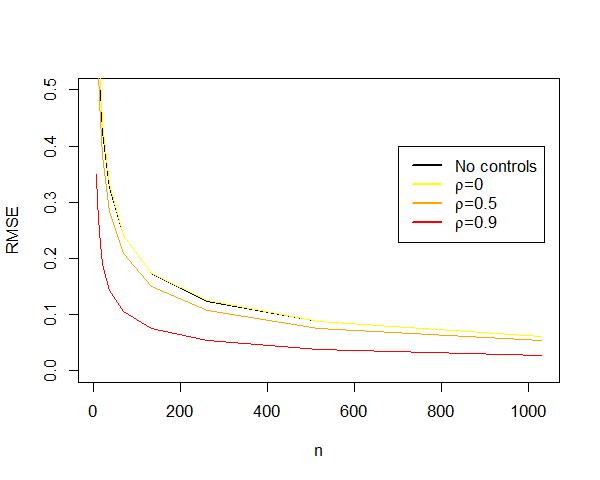
\includegraphics[width=0.65\linewidth]{figs/n}
\caption{Controls likely less important for big experiments}
\label{fig:n}
\end{figure}
\end{frame}

\begin{frame}{Conditional Bias and Precision Gains from Controls}
\protect\hypertarget{conditional-bias-and-precision-gains-from-controls-1}{}
However, including controls when treatment is correlated with covariates
can reduce ``conditional bias.'\,' Doing this will change your estimates
so be sure not to fish!

\begin{figure}
\centering
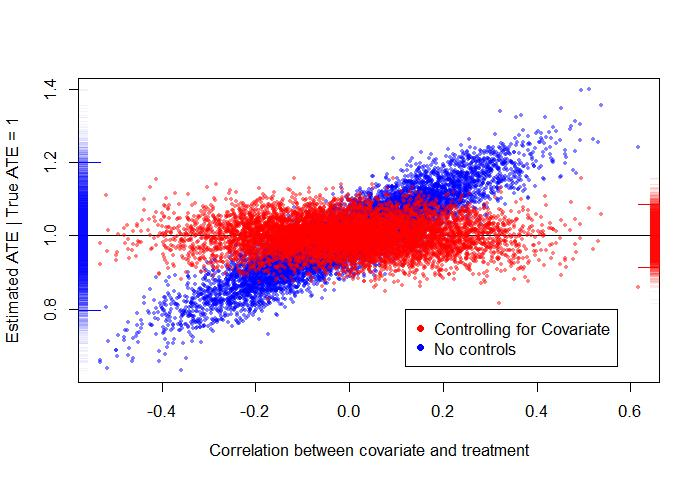
\includegraphics[width=0.7\linewidth]{figs/cb}
\caption{Advantages of controlling for vars that are correlated with outcomes}
\label{fig:cb}
\end{figure}

\#\#\{Randomization Inference\}\label{ri}
\end{frame}

\begin{frame}{Randomization Inference}
\protect\hypertarget{randomization-inference}{}
\begin{itemize}
    \item  Introducing an entirely new way to think about statistical significance\dots
    \item  Say you randomized assignment to treatment and your data looked like this.
\begin{table}
    \centering
        \begin{tabular}{l|cccccccccc}
        Unit            & 1&2&3&4&5&6&7&8&9&10\\ \hline
        Treatment & 0&0&0&0&0&0&0&1&0&0\\
        Healthy?    & 3&2&4&6&7&2&4&9&8&2\\ \hline          
        \end{tabular}
\end{table}
    \item Does the treatment improve your health?
    \item $p=$?
\end{itemize}
\end{frame}

\begin{frame}{Randomization Inference}
\protect\hypertarget{randomization-inference-1}{}
\begin{itemize}
    \item  Introducing an entirely new way to think about statistical significance\dots
    \item  Say you randomized assignment to treatment and your data looked like this.
\begin{table}
    \centering
        \begin{tabular}{l|cccccccccc}
        Unit            & 1&2&3&4&5&6&7&8&9&10\\ \hline
        Treatment & 0&0&0&0&0&0&0&1&0&0\\
        Healthy?    & 3&2&4&6&7&2&4&8&9&2\\ \hline          
        \end{tabular}
\end{table}
    \item Does the treatment improve your health?
    \item $p=$?
\end{itemize}
\end{frame}

\begin{frame}[fragile]{Randomization Inference: Some code}
\protect\hypertarget{randomization-inference-some-code}{}
\begin{itemize}
\tightlist
\item
  In principle it is very easy.
\item
  These few lines generate data, produce the regression estimate and
  then an RI estimate of \(p\):
\end{itemize}

\begin{Shaded}
\begin{Highlighting}[]
\NormalTok{X }\OtherTok{\textless{}{-}} \FunctionTok{rep}\NormalTok{(}\FunctionTok{c}\NormalTok{(}\ConstantTok{FALSE}\NormalTok{,}\ConstantTok{TRUE}\NormalTok{),}\DecValTok{50}\NormalTok{)}
\NormalTok{Y }\OtherTok{\textless{}{-}}\NormalTok{ .}\DecValTok{5}\SpecialCharTok{*}\NormalTok{X }\SpecialCharTok{+} \FunctionTok{rnorm}\NormalTok{(}\DecValTok{100}\NormalTok{)             }\CommentTok{\# DATA}

\NormalTok{b }\OtherTok{=} \FunctionTok{matrix}\NormalTok{(}\ConstantTok{NA}\NormalTok{,}\DecValTok{10000}\NormalTok{)               }\CommentTok{\# RI}
\ControlFlowTok{for}\NormalTok{(i }\ControlFlowTok{in} \DecValTok{1}\SpecialCharTok{:}\FunctionTok{length}\NormalTok{(b))\{}
\NormalTok{     Z    }\OtherTok{\textless{}{-}} \FunctionTok{sample}\NormalTok{(X)}
\NormalTok{     b[i] }\OtherTok{\textless{}{-}} \FunctionTok{mean}\NormalTok{(Y[Z])}\SpecialCharTok{{-}} \FunctionTok{mean}\NormalTok{(Y[}\SpecialCharTok{!}\NormalTok{Z])}
\NormalTok{     \}}
\FunctionTok{mean}\NormalTok{(b}\SpecialCharTok{\textgreater{}=}\FunctionTok{mean}\NormalTok{(Y[X])}\SpecialCharTok{{-}} \FunctionTok{mean}\NormalTok{(Y[}\SpecialCharTok{!}\NormalTok{X]))   }\CommentTok{\# One sided p value}
\end{Highlighting}
\end{Shaded}

{[}1{]} 0.0162
\end{frame}

\begin{frame}{Randomization Inference}
\protect\hypertarget{randomization-inference-2}{}
In practice it is a good idea to create a \(P\) matrix when you do your
randomization (although note: if the null is about one treatment, then
you are interested only in the randomization of that treatment, not the
joint randomization of all)
\end{frame}

\begin{frame}{RI (Problem revisited)}
\protect\hypertarget{ri-problem-revisited}{}
\small Return to this problem.

\begin{figure}[h]
\centering
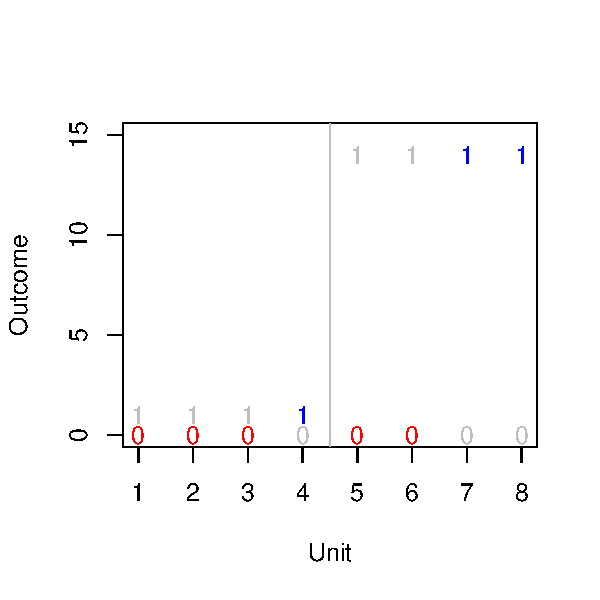
\includegraphics[width=.4\linewidth]{figs/nools}
\end{figure}

Given the strata, what are the chances that you would estimate such a
big effect if in fact there was no effect for any unit?
\end{frame}

\begin{frame}{RI (Problem revisited)}
\protect\hypertarget{ri-problem-revisited-1}{}
\small  Return to this problem.

\begin{figure}[h]
\centering
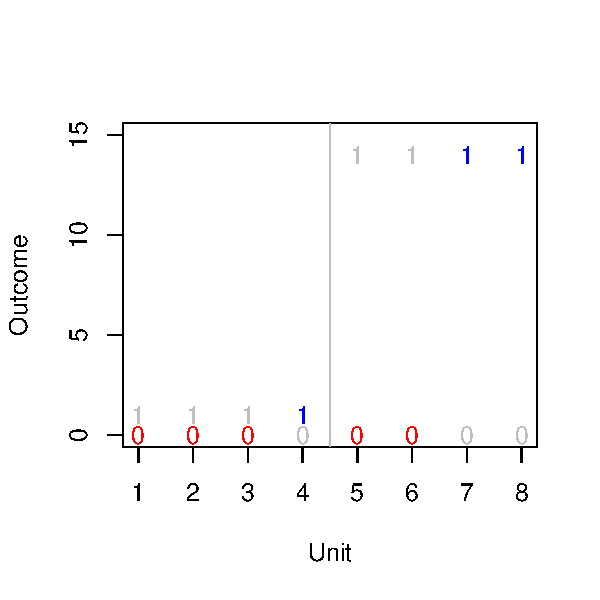
\includegraphics[width=.4\linewidth]{figs/nools}
\end{figure}

It is the probability that the two units that have Y(1)=14 both get
assigned to treatment = (1/2)*(1/3)=1/6.
\end{frame}

\begin{frame}{Randomization Inference}
\protect\hypertarget{randomization-inference-3}{}
\begin{itemize}
    \item  Say you had a silly randomization procedure and forgot to take account of it in your estimates.
        \begin{figure}[htbp]
            \centering
                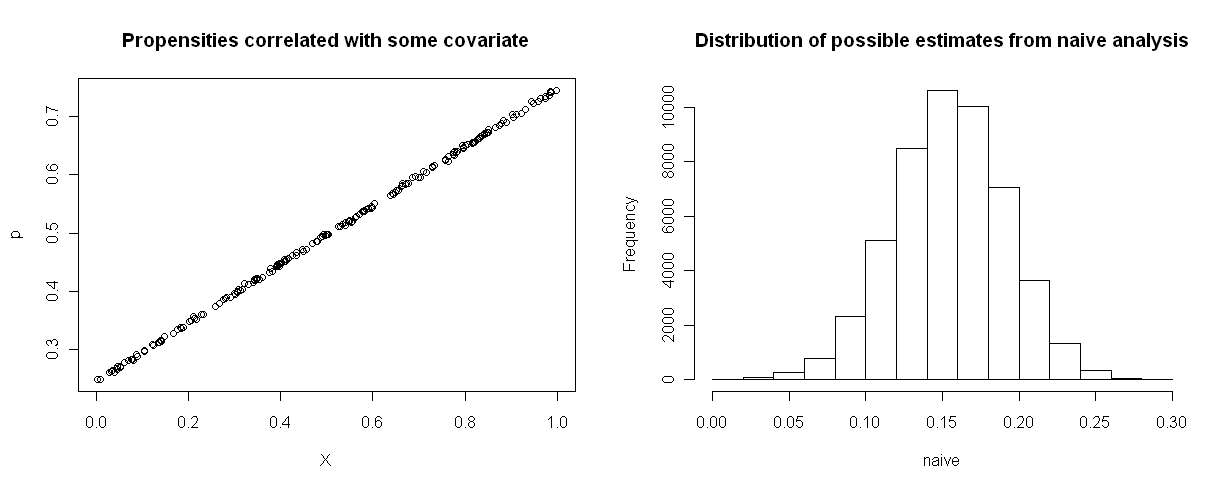
\includegraphics[width=.9\textwidth]{figs/pw2.png}
            \label{fig:pweight}
        \end{figure}
    \item You estimate .15. \textsl{Does the treatment improve your health?}
    \item $p=$?
\end{itemize}
\end{frame}

\begin{frame}{Randomization Inference}
\protect\hypertarget{randomization-inference-4}{}
\begin{itemize}
    \item  Randomization procedures are sometimes funky in lab experiments
    \item Using randomization inference would force a focus on the true assignment of individuals to treatments
    \item Fake (but believable) example follows 
\end{itemize}
\end{frame}

\begin{frame}{Randomization Inference}
\protect\hypertarget{randomization-inference-5}{}
\begin{table}
  \centering
  \caption{Optimal assignment to treatment given constraints due to facilities}
    \begin{tabular}{rrcccc}
          &       & Capacity & T1    & T2    & T3 \\ \hline
    Session & Thursday & 40    & 10    & 30    & 0 \\
          & Friday & 40    & 10    & 0     & 30 \\
          & Saturday & 10    & 10    & 0     & 0 \\ \hline
          &       & 90    & 30    & 30    & 30 \\ \hline
    \end{tabular}
\end{table}

\begin{table}[htbp] \small
  \centering
  \caption{Constraints due to subjects}
    \begin{tabular}{ccc}
    Subject Type & N     & Available \\ \hline
    A     & 30    & Thurs, Fri \\
    B     & 30    & Thurs, Sat \\
    C     & 30    & Fri, Sat \\ \hline
    \end{tabular}
\end{table}
\end{frame}

\begin{frame}{Randomization Inference}
\protect\hypertarget{randomization-inference-6}{}
\small If you think hard about assignment you might come up with an
allocation like this.

\begin{table}
  \centering
  \caption{Assignment of people to days}
    \begin{tabular}{ccc|ccc}
          &       &       &       & Allocation &  \\
    Subject Type & N     & Available & Thurs & Fri   & Sat \\ \hline
    A     & 30    & Thurs, Fri & 15    & 15    &  \\
    B     & 30    & Thurs, Sat & 25    &       & 5 \\
    C     & 30    & Fri, Sat &       & 25    & 5 \\
    \end{tabular}
\end{table}

\footnotesize  That allocation balances as much as possible. Given the
allocation you might randomly assign individuals to different days as
well as randomly assigning them to treatments within days. If you then
figure out assignment propensities, this is what you would get:

\begin{table}
  \centering
    \begin{tabular}{cccccc}
          &       &       & \multicolumn{3}{c}{Assignment Probabilities}  \\ \hline
    Subject Type & N     & Available & T1    & T2    & T3 \\ \hline
    A     & 30    & Thurs, Fri & 0.25  & 0.375 & 0.375 \\
    B     & 30    & Thurs, Sat & 0.375 & 0.625 & 0 \\
    C     & 30    & Fri, Sat & 0.375 &       & 0.625 \\ \hline
    \end{tabular}
  
\end{table}
\end{frame}

\begin{frame}{Randomization Inference}
\protect\hypertarget{randomization-inference-7}{}
\footnotesize Even under the assumption that the day of measurement does
not matter, these assignment probabilities have big implications for
analysis.

\begin{table}\footnotesize
    \begin{tabular}{ccc|ccc}
          &       &       & \multicolumn{3}{|c}{Assignment Probabilities} \\
    Subject Type & N     & Available & T1    & T2    & T3 \\ \hline
    A     & 30    & Thurs, Fri & 0.25  & 0.375 & 0.375 \\
    B     & 30    & Thurs, Sat & 0.375 & 0.625 & 0 \\
    C     & 30    & Fri, Sat & 0.375 &       & 0.625 \\
    \end{tabular}
  %
\end{table}

\begin{itemize} \footnotesize
\item Only the type $A$ subjects could have received any of the three treatments. 
\item There are no two treatments for which it is possible to compare outcomes for subpopulations $B$ and $C$
\item A comparison of $T1$ versus $T2$ can only be made for population $A \cup B$ 
\item However subpopulation $A$ is assigned to $A$ (versus $B$) with probability 4/5; while population $B$ is assigned with probability 3/8
\end{itemize}

\begin{itemize}
\item \textbf{Implications for design}: need to uncluster treatment delivery
\item \textbf{Implications for analysis}: need to take account of propensities
\end{itemize}

\color{red} \textbf{Idea}: Wacky assignments happen but if you know the
propensities you can do the analysis.

Skip to \hyperlink{subs}{\beamergotobutton{Endog Subgroups}} or
\hyperlink{ideas}{\beamerreturnbutton{Big Ideas}}
\end{frame}

\begin{frame}{Randomization Inference}
\protect\hypertarget{randomization-inference-8}{}
\begin{itemize}\small
\item Randomization inference can get quite a bit more complicated when you want to test a null other than the sharp null of no effect.
\item Say you wanted to test the null that the effect is 2 for all units. How do you do it?
\item Say you wanted to test the null that an \textit{interaction effect} is zero. How do you do it?
\item In both cases by filling in a potential outcomes schedule given the hypothesis in question and then generating a test statistic
\end{itemize}
\bigskip

\begin{table}
\centering
\begin{tabular}{cccccccc}

\multicolumn{ 2}{c}{Observed} &            & \multicolumn{ 2}{c}{Under null that } &            & \multicolumn{ 2}{c}{Under null that } \\

           &            &            & \multicolumn{ 2}{c}{effect is 0} &            & \multicolumn{ 2}{c}{effect is 2} \\  \hline

      Y(0) &       Y(1) &            &       Y(0) &       Y(1) &            &       Y(0) &       Y(1) \\

         1 &          ? &            &          1 &          1 &            &          1 &          3 \\

         2 &          ? &            &          2 &          2 &            &          2 &          4 \\

         ? &          4 &            &          4 &          4 &            &          2 &          4 \\

         ? &          3 &            &          3 &          3 &            &          1 &          3 \\

\end{tabular}  
\end{table}
\end{frame}

\hypertarget{doubly-robust-estimation}{%
\subsection{Doubly robust estimation}\label{doubly-robust-estimation}}

\begin{frame}[fragile]{Data with confounding}
\protect\hypertarget{data-with-confounding}{}
Consider this data:

\begin{Shaded}
\begin{Highlighting}[]
\CommentTok{\# df with rue treatment effect of 1 }
\CommentTok{\# (0.5 if race = 0; 1.5 if race = 1)}

\NormalTok{df }\OtherTok{\textless{}{-}}\NormalTok{ fabricatr}\SpecialCharTok{::}\FunctionTok{fabricate}\NormalTok{(}
  \AttributeTok{N =} \DecValTok{5000}\NormalTok{,}
  \AttributeTok{sex =} \FunctionTok{rep}\NormalTok{(}\DecValTok{0}\SpecialCharTok{:}\DecValTok{1}\NormalTok{, N}\SpecialCharTok{/}\DecValTok{2}\NormalTok{),}
  \AttributeTok{race =} \FunctionTok{rbinom}\NormalTok{(N, }\DecValTok{1}\NormalTok{, .}\DecValTok{5}\NormalTok{),}
  \AttributeTok{Z =} \FunctionTok{rbinom}\NormalTok{(N, }\DecValTok{1}\NormalTok{, .}\DecValTok{2} \SpecialCharTok{+}\NormalTok{ .}\DecValTok{3}\SpecialCharTok{*}\NormalTok{race),}
  \AttributeTok{Y =}\NormalTok{ .}\DecValTok{5}\SpecialCharTok{*}\NormalTok{Z }\SpecialCharTok{+}\NormalTok{ race}\SpecialCharTok{*}\NormalTok{Z }\SpecialCharTok{+}\NormalTok{ sex }\SpecialCharTok{+} \FunctionTok{rnorm}\NormalTok{(N),}
  \AttributeTok{qsmk =} \FunctionTok{factor}\NormalTok{(Z),}
  \AttributeTok{sex =} \FunctionTok{factor}\NormalTok{(sex),}
  \AttributeTok{race =} \FunctionTok{factor}\NormalTok{(race)}
\NormalTok{)}
\end{Highlighting}
\end{Shaded}
\end{frame}

\begin{frame}[fragile]{Simple approaches}
\protect\hypertarget{simple-approaches}{}
Naive regression produces biased estimates, even with controls. Lin
regression gets the right result however.

\begin{Shaded}
\begin{Highlighting}[]
\CommentTok{\# Naive}
\FunctionTok{lm\_robust}\NormalTok{(Y }\SpecialCharTok{\textasciitilde{}}\NormalTok{ Z, }\AttributeTok{data =}\NormalTok{ df)}\SpecialCharTok{$}\NormalTok{coefficients[[}\StringTok{"Z"}\NormalTok{]]}
\end{Highlighting}
\end{Shaded}

{[}1{]} 1.231162

\begin{Shaded}
\begin{Highlighting}[]
\CommentTok{\# OLS with controls}
\FunctionTok{lm\_robust}\NormalTok{(Y }\SpecialCharTok{\textasciitilde{}}\NormalTok{ Z }\SpecialCharTok{+}\NormalTok{ sex }\SpecialCharTok{+}\NormalTok{ race, }\AttributeTok{data =}\NormalTok{ df)}\SpecialCharTok{$}\NormalTok{coefficients[[}\StringTok{"Z"}\NormalTok{]]}
\end{Highlighting}
\end{Shaded}

{[}1{]} 1.13885

\begin{Shaded}
\begin{Highlighting}[]
\CommentTok{\# Lin}
\FunctionTok{lm\_lin}\NormalTok{(Y }\SpecialCharTok{\textasciitilde{}}\NormalTok{ Z,  }\SpecialCharTok{\textasciitilde{}}\NormalTok{ sex }\SpecialCharTok{+}\NormalTok{ race, }\AttributeTok{data =}\NormalTok{ df)}\SpecialCharTok{$}\NormalTok{coefficients[[}\StringTok{"Z"}\NormalTok{]]}
\end{Highlighting}
\end{Shaded}

{[}1{]} 1.030609
\end{frame}

\begin{frame}{Doubly robust estimation}
\protect\hypertarget{doubly-robust-estimation-1}{}
Doubly robust estimation combines:

\begin{enumerate}
\tightlist
\item
  A model for how the covariates predict the potential outcomes
\item
  A model for how the covariates predict assignment propensities
\end{enumerate}

Using both together to estimate potential outcomes using propensity
weighting lets you do well even if either model is wrong.

Each part can be done using nonparameteric methods resulting in an
overall semi-parametric procedure.

\begin{itemize}
\tightlist
\item
  \(\pi(Z) = \Pr(Z=1|X)\): Estimate \(\hat\pi\)
\item
  \(Y_z = \mathbb{E}[Y|Z=z, X]\): Estimate \(\hat{Y}_z\)
\item
  Estimate of causal effect:
  \(\frac{1}{n}\sum_{i=1}^n\left(\left(\frac{Z_i}{\hat{\pi}_i}(Y_i - \hat{Y}_{i1}\right) - \left(\frac{1-Z_i}{1-\hat{\pi}_i}(Y_i - \hat{Y}_{i0}\right) + \left(\hat{Y}_{i1} - \hat{Y}_{i0}\right) \right)\)
\end{itemize}
\end{frame}

\begin{frame}{Doubly robust estimation}
\protect\hypertarget{doubly-robust-estimation-2}{}
\begin{itemize}
\item
  Estimate of causal effect:
  \(\frac{1}{n}\sum_{i=1}^n\left(\left(\frac{Z_i}{\hat{\pi}_i}(Y_i - \hat{Y}_{i1}\right) - \left(\frac{1-Z_i}{1-\hat{\pi}_i}(Y_i - \hat{Y}_{i0}\right) + \left(\hat{Y}_{i1} - \hat{Y}_{i0}\right) \right)\)
\item
  Note that if \(\hat{Y}_{iz}\) are correct then the first parts drop
  out and we we get the right answer.
\item
  So if you can impute the potential outcomes, you are good (though
  hardly surprising)
\end{itemize}
\end{frame}

\begin{frame}{Doubly robust estimation}
\protect\hypertarget{doubly-robust-estimation-3}{}
\begin{itemize}
\tightlist
\item
  More subtly say the \(\hat{pi}\)s are correct, but your imputations
  are wrong; then we again have an unbiased estimator.
\end{itemize}

To see this imagine with probability \(\pi\) we assign unit 1 to
treatment and 2 to control (otherwise 1 to control and 2 to treatment).

Then our \emph{expected} estimate is:

\(\frac12\pi\left(\left(\frac{1}{\pi}(Y_{11} - \hat{Y}_{11}\right) - \left(\frac{1}{\pi}(Y_{20} - \hat{Y}_{20}\right) \right) + (1-\pi)\left(\left(\frac{1}{1-\pi}(Y_{21} - \hat{Y}_{21}\right) - \left(\frac{1}{1-\pi}(Y_{10} - \hat{Y}_{10}\right) \right) + \left(\hat{Y}_{11} - \hat{Y}_{20}\right) + \left(\hat{Y}_{21} - \hat{Y}_{10}\right)\)

\(\frac12\left(Y_{11} - Y_{10} + Y_{21}- Y_{20} +\pi\left(\left(\frac{1}{\pi}( - \hat{Y}_{11}\right) - \left(\frac{1}{\pi}( - \hat{Y}_{20}\right) \right) + (1-\pi)\left(\left(\frac{1}{1-\pi}( - \hat{Y}_{21}\right) - \left(\frac{1}{1-\pi}(- \hat{Y}_{10}\right) \right)\right) + \left(\hat{Y}_{11} - \hat{Y}_{20}\right) + \left(\hat{Y}_{21} - \hat{Y}_{10}\right)\)

\(\frac12\left(Y_{11} - Y_{10} + Y_{21}- Y_{20}\right)\)

@robins1994estimation
\end{frame}

\begin{frame}[fragile]{Doubly robust estimation}
\protect\hypertarget{doubly-robust-estimation-4}{}
\texttt{drtmle} is an R package that uses doubly robust estimation to
compute ``marginal means of an outcome under fixed levels of a
treatment.''

\begin{Shaded}
\begin{Highlighting}[]
\FunctionTok{library}\NormalTok{(SuperLearner)}
\FunctionTok{library}\NormalTok{(drtmle)}
\NormalTok{drtmle\_fit }\OtherTok{\textless{}{-}} \FunctionTok{drtmle}\NormalTok{(}
  \AttributeTok{W =}\NormalTok{ df }\SpecialCharTok{|\textgreater{}} \FunctionTok{select}\NormalTok{(sex, race), }
  \AttributeTok{A =}\NormalTok{ df}\SpecialCharTok{$}\NormalTok{Z, }
  \AttributeTok{Y =}\NormalTok{ df}\SpecialCharTok{$}\NormalTok{Y, }
  \AttributeTok{SL\_Q =} \FunctionTok{c}\NormalTok{(}\StringTok{"SL.glm"}\NormalTok{, }\StringTok{"SL.mean"}\NormalTok{, }\StringTok{"SL.glm.interaction"}\NormalTok{),}
  \AttributeTok{SL\_g =} \FunctionTok{c}\NormalTok{(}\StringTok{"SL.glm"}\NormalTok{, }\StringTok{"SL.mean"}\NormalTok{, }\StringTok{"SL.glm.interaction"}\NormalTok{),}
  \AttributeTok{SL\_Qr =} \StringTok{"SL.glm"}\NormalTok{,}
  \AttributeTok{SL\_gr =} \StringTok{"SL.glm"}\NormalTok{, }
  \AttributeTok{maxIter =} \DecValTok{1}
\NormalTok{)}
\end{Highlighting}
\end{Shaded}
\end{frame}

\begin{frame}[fragile]{Doubly robust estimation}
\protect\hypertarget{doubly-robust-estimation-5}{}
\begin{Shaded}
\begin{Highlighting}[]
\CommentTok{\# "Marginal means"}
\NormalTok{drtmle\_fit}\SpecialCharTok{$}\NormalTok{drtmle}\SpecialCharTok{$}\NormalTok{est}
\end{Highlighting}
\end{Shaded}

{[}1{]} 1.5314231 0.5001731

\begin{Shaded}
\begin{Highlighting}[]
\CommentTok{\# Effects}
\FunctionTok{ci}\NormalTok{(drtmle\_fit, }\AttributeTok{contrast =} \FunctionTok{c}\NormalTok{(}\SpecialCharTok{{-}}\DecValTok{1}\NormalTok{,}\DecValTok{1}\NormalTok{))}
\end{Highlighting}
\end{Shaded}

\$drtmle est cil ciu E{[}Y(0){]}-E{[}Y(1){]} -1.031 -1.096 -0.967

\begin{Shaded}
\begin{Highlighting}[]
\FunctionTok{wald\_test}\NormalTok{(drtmle\_fit, }\AttributeTok{contrast =} \FunctionTok{c}\NormalTok{(}\SpecialCharTok{{-}}\DecValTok{1}\NormalTok{,}\DecValTok{1}\NormalTok{))}
\end{Highlighting}
\end{Shaded}

\$drtmle zstat pval H0:E{[}Y(0){]}-E{[}Y(1){]}=0 -31.399 0

Resource: https://muse.jhu.edu/article/883477
\end{frame}

\hypertarget{assessing-performance}{%
\subsection{Assessing performance}\label{assessing-performance}}

\begin{frame}[fragile]{Assessing performance}
\textbf{Challenge}: Use \texttt{DeclareDesign} to compare performance of
\texttt{drtmle} and \texttt{lm\_lin}
\end{frame}



\end{document}
